% Manual de usuario de Micros Tempo (COOP-R14).
%
% Se compila con:   cd manual && latexmk -pdf manual.tex
% Las capturas salen de la app de verdad:   node manual/capturas.js
% (ver manual/README.md). Si una pantalla cambia, se vuelven a sacar las
% capturas y se recompila: el texto nombra los botones como dicen en
% pantalla, así que un botón que cambia de nombre se tiene que cambiar acá.
\documentclass[11pt,a4paper,oneside]{book}

\usepackage[T1]{fontenc}
\usepackage[utf8]{inputenc}
\usepackage[spanish,es-noshorthands,es-tabla]{babel}
\usepackage[scaled=0.92]{helvet}
\renewcommand{\familydefault}{\sfdefault}
\usepackage{amssymb}
\usepackage[a4paper,top=2.2cm,bottom=2.4cm,left=2.2cm,right=2.2cm,headheight=14pt]{geometry}
\usepackage{graphicx}
\usepackage[table]{xcolor}
\usepackage{microtype}
\usepackage{enumitem}
\usepackage{booktabs}
\usepackage{tabularx}
\usepackage{array}
\usepackage{fancyhdr}
\usepackage{titlesec}
\usepackage[most]{tcolorbox}
\usepackage{caption}
\usepackage[hidelinks]{hyperref}

% ─── La paleta del producto (la misma de los paneles) ───────────────────
\definecolor{tinta}{HTML}{0B2239}
\definecolor{tinta2}{HTML}{2A4864}
\definecolor{tenue}{HTML}{496A86}
\definecolor{marca}{HTML}{1668C4}
\definecolor{verde}{HTML}{1F8A4F}
\definecolor{ambar}{HTML}{A67300}
\definecolor{rojo}{HTML}{C2001D}
\definecolor{fondo}{HTML}{F4F7FB}
\definecolor{linea}{HTML}{C3D4E4}
\definecolor{verdefondo}{HTML}{E9F7EF}
\definecolor{ambarfondo}{HTML}{FDF6E4}
\definecolor{rojofondo}{HTML}{FCEBEE}

\color{tinta}
\setlength{\parindent}{0pt}
\setlength{\parskip}{6pt plus 2pt}
\linespread{1.08}

\titleformat{\chapter}[display]
  {\color{tinta}\bfseries}
  {\color{marca}\large\MakeUppercase{Capítulo \thechapter}}
  {4pt}
  {\Huge}
  [\vspace{2pt}{\color{linea}\titlerule[1pt]}]
\titlespacing*{\chapter}{0pt}{0pt}{18pt}
\titleformat{\section}{\color{tinta}\Large\bfseries}{\color{marca}\thesection}{0.6em}{}
\titleformat{\subsection}{\color{tinta2}\large\bfseries}{\color{marca}\thesubsection}{0.6em}{}
\titlespacing*{\section}{0pt}{16pt}{6pt}
\titlespacing*{\subsection}{0pt}{12pt}{4pt}

\pagestyle{fancy}
\fancyhf{}
\fancyhead[L]{\small\color{tenue}Micros Tempo · Manual de usuario}
\fancyhead[R]{\small\color{tenue}\nouppercase{\leftmark}}
\fancyfoot[C]{\small\color{tenue}\thepage}
\renewcommand{\headrulewidth}{0.4pt}
\renewcommand{\headrule}{{\color{linea}\hrule width\headwidth height\headrulewidth}}
\fancypagestyle{plain}{\fancyhf{}\fancyfoot[C]{\small\color{tenue}\thepage}\renewcommand{\headrulewidth}{0pt}}

\captionsetup{font={small,color=tenue},labelfont={bf,color=tinta2},labelsep=period}
\setlist{itemsep=2pt,topsep=4pt,leftmargin=1.4em}

% ─── Piezas de texto ────────────────────────────────────────────────────
% Un botón o un rótulo, como se lee en pantalla
\newcommand{\boton}[1]{\tcbox[on line,boxsep=0pt,left=3pt,right=3pt,top=1.5pt,bottom=1.5pt,
  colback=white,colframe=linea,boxrule=0.5pt,arc=2pt]{\footnotesize\bfseries\color{tinta2}#1}}
\newcommand{\rotulo}[1]{{\footnotesize\bfseries\color{tinta2}\MakeUppercase{#1}}}
\newcommand{\enverde}[1]{{\color{verde}\bfseries #1}}
\newcommand{\enambar}[1]{{\color{ambar}\bfseries #1}}
\newcommand{\enrojo}[1]{{\color{rojo}\bfseries #1}}
\newcommand{\flecha}{$\rightarrow$\ }
\newcommand{\idavuelta}{$\rightleftarrows$}

\newtcolorbox{importante}[1][Importante]{enhanced,breakable,colback=rojofondo,colframe=rojo,
  boxrule=0pt,leftrule=3pt,arc=2pt,left=8pt,right=8pt,top=5pt,bottom=5pt,
  title={\bfseries #1},coltitle=rojo,colbacktitle=rojofondo,attach title to upper={\ \ }}
\newtcolorbox{consejo}[1][Consejo]{enhanced,breakable,colback=verdefondo,colframe=verde,
  boxrule=0pt,leftrule=3pt,arc=2pt,left=8pt,right=8pt,top=5pt,bottom=5pt,
  title={\bfseries #1},coltitle=verde,colbacktitle=verdefondo,attach title to upper={\ \ }}
\newtcolorbox{nota}[1][Para saber]{enhanced,breakable,colback=ambarfondo,colframe=ambar,
  boxrule=0pt,leftrule=3pt,arc=2pt,left=8pt,right=8pt,top=5pt,bottom=5pt,
  title={\bfseries #1},coltitle=ambar,colbacktitle=ambarfondo,attach title to upper={\ \ }}

% ─── Capturas ───────────────────────────────────────────────────────────
\setlength{\fboxsep}{0pt}
\setlength{\fboxrule}{0.6pt}
% Pantalla de teléfono, en una fila de dos o tres
\newcommand{\cel}[3][0.31]{%
  \begin{minipage}[t]{#1\textwidth}\centering
    \fcolorbox{linea}{white}{\includegraphics[width=0.96\linewidth]{img/#2}}\par\vspace{3pt}
    {\footnotesize\color{tenue}#3}
  \end{minipage}}
% Pantalla de escritorio, con su número de figura
\newcommand{\pc}[3][1]{%
  \begin{figure}[htbp]\centering
    \fcolorbox{linea}{white}{\includegraphics[width=\dimexpr#1\textwidth-2\fboxrule\relax]{img/#2}}
    \caption{#3}\label{fig:#2}
  \end{figure}}

\begin{document}
\frontmatter

% ─── Portada ────────────────────────────────────────────────────────────
\begin{titlepage}
  \newgeometry{margin=0pt}
  \pagecolor{tinta}\color{white}
  \vspace*{5.5cm}
  \hspace*{2.4cm}\begin{minipage}{0.75\paperwidth}
    {\large\color{marca!45!white}\bfseries CONTROL DE FLOTA PARA COOPERATIVAS DE TRANSPORTE}\par\vspace{14pt}
    {\fontsize{46}{50}\selectfont\bfseries Micros Tempo}\par\vspace{10pt}
    {\fontsize{24}{28}\selectfont Manual de usuario}\par\vspace{28pt}
    {\large Para el chofer, el cobrador, Despacho, la gerencia\\y la central que administra el sistema.}\par
    \vspace{5.5cm}
    {\color{marca!45!white}Versión de octubre de 2026 · app Android versión 5}\par\vspace{4pt}
    {\color{marca!45!white}soporte@microstempo.com}
  \end{minipage}
  \restoregeometry
\end{titlepage}
\nopagecolor\color{tinta}

\chapter*{Cómo leer este manual}
\addcontentsline{toc}{chapter}{Cómo leer este manual}

Micros Tempo tiene cuatro pantallas, una por cada persona que lo usa. No hace
falta leer el manual entero: cada uno va a su capítulo.

\begin{center}
\renewcommand{\arraystretch}{1.35}
\begin{tabularx}{\textwidth}{>{\bfseries}l X >{\raggedright\arraybackslash}p{4.3cm}}
\toprule
\rowcolor{fondo} Quién & Para qué lo usa & Dónde leer \\
\midrule
Chofer & Mirar de reojo, manejando, cuánto le lleva la combi de adelante y la de atrás; avisar tráfico; pedir ayuda; hablar con la ruta y con Despacho. & Capítulos \ref{cap:ideas} y \ref{cap:chofer} \\
Cobrador & Lo mismo que el chofer, desde su propio celular, sin que su GPS cuente. & Capítulo \ref{cap:cobrador} \\
Despacho & Operar el día: ver la flota en el mapa, atender emergencias, escribirle a una combi, dar de alta a la gente, sacar informes. & Capítulos \ref{cap:ideas} y \ref{cap:despacho} \\
Gerencia & Todo lo de Despacho más los números del período, las combis y los datos de la empresa. & Capítulo \ref{cap:gerencia} \\
Central & Dar de alta cooperativas, dibujar sus recorridos, respaldar la base y mirar la salud del sistema. & Capítulo \ref{cap:central} \\
\bottomrule
\end{tabularx}
\end{center}

Las capturas son del sistema funcionando, con una cooperativa inventada para el
manual: \emph{Transportes Altiplano}, con dos rutas por calles de Juliaca
(la 18A, \emph{Norte \idavuelta{} Taparachi}, y la 18B), doce combis y catorce
personas. Los nombres, placas y números son de mentira.

Los nombres de los botones van \boton{ASÍ}, tal como se leen en pantalla.

\tableofcontents

\mainmatter

% ════════════════════════════════════════════════════════════════════════
\chapter{Antes de empezar}
\label{cap:antes}

\section{Qué es Micros Tempo}

Micros Tempo mide, en vivo, la \textbf{separación en minutos} entre las combis
de una misma ruta, y se la muestra a cada chofer en grande: cuánto le lleva la
de adelante y cuánto la de atrás. El objetivo es que las combis salgan
parejas —ni pegadas una a la otra (el \emph{pelotón}, que se reparte los
pasajeros y deja paraderos vacíos) ni muy separadas—.

Además, la cooperativa ve la flota entera en un mapa, recibe las emergencias
al instante, habla con cada combi y cuenta las vueltas, las horas y el
cumplimiento de cada unidad, sin planillas.

\section{Qué hace falta}

\begin{itemize}
  \item \textbf{Chofer y cobrador:} un celular Android con GPS y datos móviles.
    Lo mejor es la \textbf{app Android}, que sigue mandando la posición con la
    pantalla apagada. También se puede usar la \textbf{web del chofer} desde el
    navegador del celular, pero ahí la pantalla tiene que quedar encendida.
  \item \textbf{Despacho, gerencia y central:} una computadora con un navegador
    actualizado (Chrome, Edge o Firefox) e internet. El panel también abre en
    una tablet.
  \item \textbf{Usuario y clave} para cada persona. A los choferes y cobradores
    se los da Despacho; a Despacho y a la gerencia, la central.
\end{itemize}

\section{Dónde se entra}

Todo vive en una misma dirección de internet, la que entrega la central al dar
de alta la cooperativa. Por ejemplo, si la dirección es
\texttt{https://flota.ejemplo.pe}:

\begin{center}
\renewcommand{\arraystretch}{1.3}
\begin{tabular}{>{\bfseries}l l}
\toprule
\rowcolor{fondo} Pantalla & Dirección \\
\midrule
Web del chofer y del cobrador & \texttt{https://flota.ejemplo.pe/} \\
Panel de Despacho y de gerencia & \texttt{https://flota.ejemplo.pe/despacho.html} \\
Panel de la central & la que configure la central (por defecto \texttt{/creador}) \\
\bottomrule
\end{tabular}
\end{center}

\begin{consejo}
En el celular, la web del chofer se puede \textbf{instalar como una app}: en
Chrome, menú \flecha \emph{Agregar a la pantalla principal}. Abre a pantalla
completa y, si una vez se cargó, abre aunque no haya señal.
\end{consejo}

% ════════════════════════════════════════════════════════════════════════
\chapter{Las ideas que hay que conocer}
\label{cap:ideas}

Cinco ideas explican casi todo lo que muestran las pantallas. Vale la pena
leerlas una vez, aunque se use sólo el panel de Despacho.

\section{La brecha}

La \textbf{brecha} es cuántos minutos de recorrido separan a una combi de la
que va adelante (\rotulo{adelante}) y de la que viene atrás (\rotulo{atrás}),
en el mismo sentido de la ruta. No es la distancia en línea recta: se mide
sobre el recorrido dibujado de la ruta, y se convierte a minutos con la
duración de punta a punta de esa ruta.

Cada ruta tiene un \textbf{objetivo de brecha}: la separación ideal. Lo fija
Despacho a mano, o lo calcula el sistema solo (la vuelta promedio dividida por
las combis que hay en ruta). Cada brecha se pinta según cuánto se aparta del
objetivo:

\begin{center}
\renewcommand{\arraystretch}{1.35}
\begin{tabularx}{\textwidth}{l l X}
\toprule
\rowcolor{fondo} Color & Palabra & Qué quiere decir \\
\midrule
\enverde{Verde} & \rotulo{en objetivo} & A no más de un 15\,\% del objetivo. Con un objetivo de 6:00, entre 5:06 y 6:54. \\
\enambar{Ámbar} & \rotulo{al límite} & Entre un 15 y un 30\,\% de diferencia. Hay que corregir de a poco. \\
\enrojo{Rojo} & \rotulo{crítica} & Más de un 30\,\% de diferencia. Si es por pegarse a la de adelante, es el \emph{pelotón}. \\
\bottomrule
\end{tabularx}
\end{center}

El color nunca va solo: al lado siempre está la palabra, para que se entienda
también con el sol de frente o sin distinguir colores.

\section{La cadena: en ruta, yendo, ausente, fuera}

Sólo se miden entre sí las combis que están \textbf{en la cadena}: las que el
chofer declaró en ruta \emph{y} que el GPS ya vio sobre el recorrido. Lo que
declara el chofer es su \textbf{presencia}:

\begin{description}[leftmargin=0pt,labelsep=0.6em,itemsep=4pt]
  \item[En ruta.] Salió a trabajar. Mientras el GPS todavía no lo ve sobre el
    recorrido (viene de su casa, del grifo), la pantalla dice
    \enambar{YENDO A LA RUTA}: su brecha y su vuelta arrancan recién al pisar
    el trazado.
  \item[Ausente.] Para comer, buscar un repuesto, un descanso. La combi sigue
    en el mapa de Despacho, pero sale de la cadena: nadie se mide contra ella
    y la vuelta que llevaba se descarta.
  \item[Fuera.] Terminó. La combi se va del mapa en el acto.
\end{description}

\section{La ida, el retorno y la vuelta}

Cada ruta tiene una \textbf{ida} y un \textbf{retorno} (o \emph{vuelta}),
dibujados por separado: el primer punto de cada uno es el paradero inicial.
Las brechas se miden sólo entre combis del mismo tramo: la última de la ida no
se mide contra la primera del retorno.

Una \textbf{vuelta} es el circuito entero, ida y retorno. El sistema la cuenta
sola al cruzar el paradero inicial, con su duración y la brecha promedio que
mantuvo. Si una combi se mete a la ruta ya empezada (más allá del 15\,\% del
circuito), su primera vuelta queda marcada como \textbf{parcial}: se guarda,
pero no entra en los promedios, y Despacho la ve marcada como \enambar{ENTRÓ
\textit{n}\,\%}. Las idas y los retornos sueltos también se cuentan.

\section{Lo que puede pasarle a una combi}

\begin{description}[leftmargin=0pt,labelsep=0.6em,itemsep=4pt]
  \item[Sin señal.] Hace más de 30 segundos que no llega su posición: se ve en
    gris, con la hora de su última posición. A las que vienen detrás se les
    avisa que adelante hay alguien sin señal, en lugar de dejarlas apurarse
    hacia una combi que no ven.
  \item[Fuera del recorrido.] Se alejó del trazado más de lo permitido (300 m
    por defecto) y se sostuvo. Despacho lo ve y puede silenciarlo si ya sabe el
    motivo (una obra, un desfile).
  \item[En tráfico.] El chofer avisó que está trabado, o el sistema vio que en
    tres minutos casi no avanzó. A la que viene atrás se le dice que no se
    apure hacia el embotellamiento.
\end{description}

\section{El SOS}

El botón de emergencia se \textbf{desliza}, no se toca: así no sale por
accidente. La alerta sale en el acto a Despacho y a todas las combis de la
ruta, con la posición. Después, si puede, el chofer elige qué pasó (falla
mecánica, accidente, policía); si no elige, queda como SOS a secas.

% ════════════════════════════════════════════════════════════════════════
\chapter{El chofer}
\label{cap:chofer}

La pantalla del chofer está pensada para mirarse un segundo, de reojo, con el
celular en el soporte y el sol de frente. Las capturas son de la web del
chofer; la app Android tiene las mismas pantallas y algunas cosas más
(sección \ref{sec:android}).

\section{Entrar}

Se entra con el usuario y la clave que da Despacho. La pantalla dice si hay
conexión con el servidor (\enverde{CONECTADO}). El celular recuerda el último
usuario: al día siguiente sólo hace falta la clave.

\begin{center}
\cel{c01-entrar}{Entrar.}\hfill
\cel{c13-olvide}{«Olvidé mi contraseña».}\hfill
\cel{c02-puerta}{La puerta: ¿salir a ruta?}
\end{center}

Si se olvidó la clave, \boton{Olvidé mi contraseña} explica qué hacer: la clave
nueva la pone Despacho (o, para un cobrador, el chofer de su combi desde la
app Android). No hay recuperación por correo.

\section{La puerta: ¿salir a ruta ahora?}

Después de entrar aparece la \textbf{puerta}. Muestra quién entró, la unidad
y la ruta, y dos opciones:

\begin{itemize}
  \item \boton{SALIR A RUTA \flecha} empieza el turno: la combi aparece en el
    mapa y empieza a emitir su posición.
  \item \boton{Entrar AUSENTE (comer, un repuesto)} entra sin salir a ruta. Se
    habilita a los 15 segundos, a propósito: es para cuando de verdad se va a
    estar parado.
\end{itemize}

Arriba a la derecha, \boton{Salir} cierra la sesión.

\subsection{¿En qué combi salís?}

\begin{minipage}[t]{0.64\textwidth}\vspace{0pt}
Si Despacho te habilitó más de una combi, la puerta pregunta
\rotulo{¿En qué combi salís?}. Cada una dice si está \emph{libre} o quién
la maneja ahora; la elegida está marcada (\rotulo{ELEGIDA}). Se toca la otra y
listo: pasa a ser la tuya de hoy, y la ruta va con la combi.

Elegir \textbf{no le saca nada a nadie}: la combi se toma al salir a ruta. Si
elegís una que está manejando otro, la app lo nombra y pide confirmar:
\boton{ES UN RELEVO}. Al salir a ruta la tomás vos y al otro le aparece que
otro chofer tomó la unidad.

Estando en ruta no se cambia de combi: primero \boton{SALIR DE RUTA}.
\end{minipage}\hfill
\begin{minipage}[t]{0.3\textwidth}\vspace{0pt}\centering
\cel[1]{c02c-relevo}{Elegir la que maneja otro pide confirmar el relevo.}
\end{minipage}

\textbf{Entrar no es salir.} Poner la clave no cuenta horas ni le saca la
combi a nadie: el turno arranca al tocar \boton{SALIR A RUTA} (o
\boton{Entrar AUSENTE}). Mientras tanto, Despacho ve al chofer en la lista de
\textbf{los que entraron y no salieron a ruta}.

\subsection{Si arrancás sin salir a ruta}

\begin{minipage}[t]{0.64\textwidth}\vspace{0pt}
En la puerta el teléfono no manda la ubicación. Pero con la app abierta la
\textbf{mira}, sin mandarla, y se da cuenta si la combi ya está andando: lejos
de donde entraste y a velocidad de combi, sostenida (caminar o un salto del
GPS no cuentan). Entonces avisa fuerte, con vibración:
\enambar{¿YA ESTÁS MANEJANDO?}, con una cuenta regresiva.

\begin{itemize}
  \item Si no tocás nada, \textbf{al minuto sale a ruta sola}, y Despacho lo ve
    en la Actividad.
  \item \boton{SALIR AHORA} (en la web) sale en el acto; en la app Android se
    sigue deslizando.
  \item \boton{No estoy manejando} (vas de pasajero, te llevan) lo calla media
    hora.
\end{itemize}

Mira sólo con la app abierta y con el permiso de ubicación ya dado: no lo
pide en la puerta.
\end{minipage}\hfill
\begin{minipage}[t]{0.3\textwidth}\vspace{0pt}\centering
\cel[1]{c02b-vigia}{¿Ya estás manejando?}
\end{minipage}

\section{Yendo a la ruta}

Al salir a ruta, mientras el GPS todavía no ve la combi sobre el recorrido, la
pantalla lo dice en ámbar: \enambar{YENDO A LA RUTA}. No es una falla: la
brecha y la vuelta arrancan al pisar el trazado. Así, marcar desde la casa no
confunde a nadie.

\begin{center}
\cel{c04-yendo}{Yendo a la ruta.}\hfill
\cel{c03-brechas}{En ruta: las dos brechas en objetivo.}\hfill
\cel{c05-trafico}{Avisando tráfico.}
\end{center}

\section{La pantalla de brechas}
\label{sec:brechas}

Es la pantalla principal, la del medio. De arriba hacia abajo:

\begin{enumerate}
  \item \textbf{La barra de color} del borde superior: el estado de la brecha
    más importante, para verlo con el rabillo del ojo.
  \item \rotulo{En vivo · 7}: hay conexión, y cuántas combis están en la
    cadena de la ruta (el mismo número que ve Despacho). A la derecha, la
    velocidad.
  \item \textbf{La brecha grande}: la que más importa en este momento
    (\rotulo{adelante} o \rotulo{atrás}), con la combi contra la que se mide
    (\emph{+1 · M-03} es la de adelante; \emph{\mbox{-1} · M-02}, la de atrás).
  \item \textbf{La instrucción}, en una línea.
  \item \textbf{La otra brecha}, más chica. \rotulo{OK} si está en objetivo.
  \item Los botones \boton{ESTOY EN TRÁFICO}, \boton{AUSENTE} y
    \boton{SALIR DE RUTA}, y el \textbf{SOS} deslizable.
\end{enumerate}

Lo que puede decir la instrucción:

\begin{center}
\renewcommand{\arraystretch}{1.3}
\begin{tabularx}{\textwidth}{>{\raggedright\arraybackslash}p{6.3cm} X}
\toprule
\rowcolor{fondo} Mensaje & Qué hacer \\
\midrule
Mantené el ritmo. Objetivo 6:00. & Nada: la brecha está en objetivo. \\
Apurá un poco. Objetivo 6:00. & La de adelante se escapa, o la de atrás te viene pisando. \\
Aflojá un poco. Objetivo 6:00. & Vas encima de la de adelante, o la de atrás quedó lejos. \\
M-05 avisa que está en tráfico 4 min. Mantené: no te apures hacia el embotellamiento. & La de adelante está trabada: su brecha crece sola, no la persigas. \\
M-05 se quedó sin señal. Andá con cuidado: sigue en ruta. & Hay una combi adelante que no se ve en el mapa. \\
Sos la única unidad en ruta. & No hay con quién medirse. \\
\bottomrule
\end{tabularx}
\end{center}

Deslizando a los costados (o tocando los puntos de arriba) se pasa al
\textbf{chat} (izquierda) y al \textbf{mapa} (derecha).

\section{Día, noche o automático}

\begin{minipage}[t]{0.64\textwidth}\vspace{0pt}
Arriba a la derecha, en las tres pantallas, está el botón del tema. Cada toque
pasa al siguiente: \boton{AUTO} \flecha \boton{DÍA} \flecha \boton{NOCHE}.

\begin{itemize}
  \item \boton{DÍA} viene de fábrica: fondo claro, el que mejor se lee con el
    sol de frente.
  \item \boton{NOCHE}: fondo negro, para no encandilar manejando de noche.
  \item \boton{AUTO}: de día hasta las 18:30 y de noche hasta las 5:30. Cambia
    solo, sin tocar nada.
\end{itemize}

El teléfono se acuerda de lo elegido. En la app Android el botón está en la
barra de abajo y viene en \boton{AUTO}; su noche, además, tira a ámbar, con
menos azul.
\end{minipage}\hfill
\begin{minipage}[t]{0.3\textwidth}\vspace{0pt}\centering
\cel[1]{c15-noche}{La pantalla de brechas en NOCHE.}
\end{minipage}

\section{Estoy en tráfico}

Un toque en \boton{ESTOY EN TRÁFICO} avisa a la ruta que la combi está
trabada: a la que viene atrás se le cambia la instrucción a «mantené». El botón
queda en ámbar, \boton{EN TRÁFICO · TOCÁ PARA QUITAR}, y se apaga solo cuando
la combi vuelve a andar. Si el sistema nota que la combi lleva un rato casi
quieta, el botón pregunta \boton{¿ESTÁS EN TRÁFICO? · TOCÁ PARA AVISAR}.

\section{Ausente}

\boton{AUSENTE} saca a la combi de la cadena sin sacarla del mapa: para comer,
para buscar un repuesto. Arriba queda un cartel ámbar con
\boton{VOLVER A RUTA}, y la pantalla lo dice claro: nadie se mide contra uno
y la vuelta que llevaba quedó descartada.

\begin{center}
\cel{c06-ausente}{Ausente.}\hfill
\cel{c07-salir-confirmar}{Salir de ruta pide un segundo toque.}\hfill
\cel{c08-sos-enviado}{SOS: alerta enviada.}
\end{center}

\section{Salir de ruta}

\boton{SALIR DE RUTA} termina el turno: la combi se va del mapa de todos en el
acto. Por eso pide \textbf{un segundo toque}: el botón se pone rojo y dice
\boton{¿SEGURO? TOCÁ DE NUEVO}. Si no se toca en unos segundos, se desarma
solo. Después de salir se vuelve a la puerta.

\subsection{El relevo}

Cuando otro chofer sube a la combi y toca \boton{SALIR A RUTA}, la combi pasa
a ser de él: su teléfono manda la posición y su turno arranca; el del que
bajó se cierra, y a éste le aparece \enambar{Otro chofer tomó la unidad}.
Despacho lo ve en la Actividad.

El que bajó \textbf{no recupera la combi solo}, aunque le quede la app abierta
y se reconecte en su casa, y aunque el otro termine el turno. Para volver a
manejarla tiene que hacerlo a propósito: \boton{SALIR DE RUTA} y después
\boton{SALIR A RUTA}, o volver a entrar con su usuario y clave.

\section{SOS}
\label{sec:sos}

Para pedir ayuda, \textbf{deslizar} el cuadrado rojo \boton{SOS} hacia la
derecha hasta el final. La pantalla se pone roja y dice
\enrojo{ALERTA ENVIADA} \emph{recién cuando el servidor la recibió}; si no
salió, dice que no salió y hay que repetir.

Enseguida aparece \textbf{¿Qué pasó?} con tres botones: \boton{FALLA MECÁNICA},
\boton{ACCIDENTE} y \boton{POLICÍA}. Elegir uno le dice a Despacho si mandar una
grúa o una ambulancia. Es opcional: \boton{Cerrar — queda como SOS} o no tocar
nada deja la alerta como SOS a secas.

\begin{center}
\cel[0.36]{c09-sos-que-paso}{¿Qué pasó? — después de la alerta.}\hfill
\cel[0.36]{c10-mapa}{El mapa.}
\end{center}

\begin{importante}
El SOS sale aunque el GPS no tenga posición. Si el celular no tiene señal en
ese momento, la pantalla lo dice: \textbf{no supongas que llegó} si no viste
\enrojo{ALERTA ENVIADA}.
\end{importante}

\section{El mapa}

El mapa muestra la combi propia (\textbf{TÚ}), el recorrido de la ruta (la ida
con línea llena, el retorno punteado) y las otras combis. Abajo queda siempre
la tarjeta con las dos brechas, para no perder el dato. Arriba, la ruta y
cuántas combis hay en la cadena.

\section{El chat}

A la izquierda de la pantalla de brechas está el chat, con tres canales:

\begin{itemize}
  \item \boton{GRUPO 18A}: toda la ruta. Lo leen todas las combis de la ruta y
    Despacho.
  \item \boton{COMBI M-01}: lo que Despacho habla \textbf{con la combi}. Lo ven
    el chofer y el cobrador que van arriba, y el que la maneje después. Es
    para lo de la calle: \emph{esperá en el mercado}.
  \item \boton{PERSONAL}: lo que hablás \textbf{solo vos con Despacho}. Te
    sigue aunque cambies de combi, y no lo ve nadie más: ni tu cobrador, ni el
    que maneje tu combi después. Es para lo tuyo: \emph{pasá por la oficina}.
\end{itemize}

Un chofer no puede escribirle en privado a otro chofer. Cada pestaña con
algo sin leer muestra cuántos.

Se escribe abajo y se manda con la flecha. El botón del micrófono graba una
\textbf{nota de voz}: se mantiene apretado mientras se habla y se suelta para
enviar. Los mensajes de otro día llevan la fecha (\emph{21/10 09:18}).

\begin{center}
\cel{c11-chat-grupo}{El grupo de la ruta.}\hfill
\cel{c12-chat-despacho}{Despacho a la combi.}\hfill
\cel{c12b-chat-personal}{Despacho, sólo a Rufino.}
\end{center}

\section{La app Android}
\label{sec:android}

La app Android tiene las mismas pantallas, y además:

\begin{itemize}
  \item \textbf{Manda la posición con la pantalla apagada}, todo el turno. La
    web, en cambio, necesita la pantalla encendida.
  \item \textbf{La brecha en la notificación}: se puede mirar sin abrir la app.
  \item \textbf{Ausente inteligente}: si el chofer se olvidó de volver a ruta
    después de almorzar, vuelve solo al alejarse 300 m; y una ausencia de más
    de 2 horas pasa a \emph{fuera} sola.
  \item \textbf{Perfil}: sus vueltas, horas y cumplimiento de 7 o 30 días, sus
    turnos, su alias y su clave.
  \item \textbf{Sus cobradores}: el chofer ve a los cobradores de su combi, les
    cambia la clave y los saca (darlos de alta sigue siendo de Despacho).
  \item \textbf{Grabar recorrido}: Perfil \flecha \boton{GRABAR RECORRIDO}
    guarda el camino que maneja, para que la central lo use al dibujar la ruta.
  \item \textbf{Fotos} en el chat, además de las notas de voz.
\end{itemize}

\begin{nota}[La batería]
Para que la app siga mandando la posición con la pantalla apagada, Android
tiene que dejarla correr sin \emph{optimización de batería}. Si está activada,
la app lo dice en rojo y tiene un atajo a los ajustes. En algunos teléfonos
(Xiaomi, Huawei, Oppo) además hay que permitir el \emph{inicio automático}.
\end{nota}

% ════════════════════════════════════════════════════════════════════════
\chapter{El cobrador}
\label{cap:cobrador}

El cobrador entra con \textbf{su propia cuenta} (nunca con la del chofer) y ve
lo mismo que el chofer de su combi: las brechas, el mapa y el chat del grupo y
de Despacho. La diferencia está arriba: \rotulo{acompañante}. Su GPS
\textbf{no} cuenta: la posición de la combi la manda el celular del chofer.

\begin{center}
\cel[0.36]{c14-cobrador}{El cobrador, en modo acompañante.}
\end{center}

Puede usar el SOS: si su celular no tiene posición, la alerta sale con la
posición de su combi. Si se olvidó la clave, se la cambia Despacho o el chofer
de su combi (desde la app Android).

% ════════════════════════════════════════════════════════════════════════
\chapter{Despacho}
\label{cap:despacho}

El panel de Despacho es la pantalla de la operación del día. Está pensado para
estar abierto todo el turno en una computadora.

\section{Entrar}

Se entra en \texttt{/despacho.html} con el usuario y la clave de Despacho. Si
se olvidó la clave, la restablece la central. Con la misma pantalla entra la
gerencia (capítulo \ref{cap:gerencia}).

\pc[0.7]{d01-entrar}{La entrada al panel de Despacho y de gerencia.}

\section{El panel}

\pc{d02-panel}{El panel de Despacho con la flota andando.}

La figura \ref{fig:d02-panel} es el panel con la ruta 18A en marcha. Tiene
cuatro partes:

\begin{description}[leftmargin=0pt,labelsep=0.6em,itemsep=4pt]
  \item[La cabecera.] El nombre y el logo de la cooperativa; el selector de
    \textbf{ruta} (el supervisor ve todas las de la cooperativa); el estado,
    \rotulo{en vivo · 7 en ruta · 1 sin señal · 1 ausente}; el
    \textbf{objetivo de brecha} vigente; \boton{Gestión}, el botón de la luna (el tema
    noche) y \boton{Salir}.
  \item[La lista de unidades.] A la izquierda, cada combi con su velocidad,
    chofer, placa, tramo (\rotulo{ida} / \rotulo{vuelta}) y sus dos brechas,
    con color y palabra. Arriba, \rotulo{8 de 8}: cuántas se ven de cuántas
    tiene la ruta. Encima de la lista, dos avisos cuando hace falta: las
    combis \textbf{fuera del recorrido} y los choferes que \textbf{entraron y
    no salieron a ruta}, con hace cuánto; a los diez minutos se pone en
    ámbar: es para llamarlo.
  \item[El mapa.] El recorrido (ida llena, retorno punteado), las combis con
    el color de su brecha y la leyenda. Una combi \textbf{fuera del recorrido}
    lleva un rombo y un círculo ámbar.
  \item[El canal de la ruta.] A la derecha, el chat del grupo, con los SOS
    marcados en rojo. Abajo se escribe al canal.
\end{description}

\section{Lo que dice cada tarjeta}

\begin{minipage}[t]{0.3\textwidth}\vspace{0pt}
\fcolorbox{linea}{white}{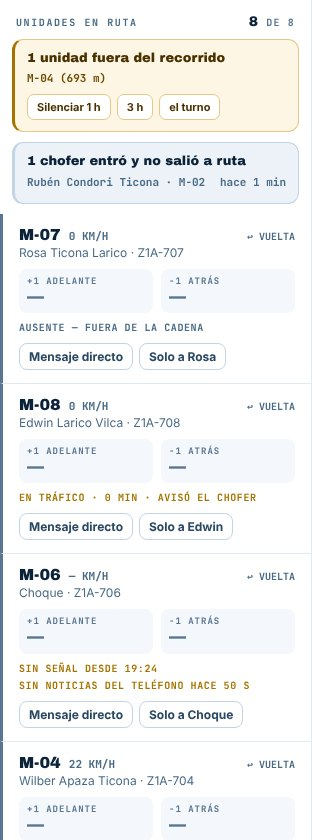
\includegraphics[width=\dimexpr\linewidth-2\fboxrule\relax]{img/d03-lista}}
\end{minipage}\hfill
\begin{minipage}[t]{0.66\textwidth}\vspace{0pt}
Debajo de las brechas, cada tarjeta puede llevar un aviso:

\begin{itemize}
  \item \enambar{AUSENTE — FUERA DE LA CADENA}: el chofer se declaró ausente.
  \item \enambar{EN TRÁFICO · 4 MIN · AVISÓ EL CHOFER}: trabada. Si no lo avisó
    el chofer, dice \emph{parada}: lo midió el sistema.
  \item \enambar{SIN SEÑAL DESDE 21:56}: no llega su posición. La línea de
    abajo distingue \emph{sin noticias del teléfono} (no llega nada: la combi
    puede estar en un lugar sin cobertura) de \emph{el teléfono sigue mandando}
    (llega, pero con posiciones viejas: es un problema del celular, no de la
    calle). Una combi sin señal no muestra brechas: su posición es vieja.
  \item \enambar{$\hookrightarrow$\ ENTRÓ 46\,\%}: se metió a la ruta ya empezada.
  \item \enambar{GPS SOSPECHOSO · motivo}: las posiciones tienen la firma de un
    GPS simulado. Es una sospecha, para preguntar; no acusa a nadie.
  \item \enambar{RELOJ ATRASADO}: la hora del celular está corrida; el sistema
    ya lo corrige.
\end{itemize}

Arriba de la lista, un recuadro ámbar avisa las combis \textbf{fuera del
recorrido}, con cuántos metros. \boton{Silenciar 1 h}, \boton{3 h} y
\boton{el turno} lo callan cuando ya se sabe el motivo: silenciar es «ya lo
sé», no «no pasó», y queda registrado.

Cada tarjeta tiene \boton{Mensaje directo}.
\end{minipage}

\section{Escribirle a una combi o a una persona}

Hay dos privados, y no son lo mismo:

\begin{itemize}
  \item \boton{Mensaje directo} en la tarjeta de una combi abre la
    conversación \textbf{con esa combi}: la ven su chofer y su cobrador (en su
    canal \boton{COMBI}) y quien la maneje después. Arriba dice
    \rotulo{toda esa combi}. Es para lo de la calle.
  \item \boton{Solo a Rufo} (el que la maneja ahora) abre la conversación
    \textbf{con esa persona}: la sigue a cualquier combi, y no la ve nadie más
    —ni su cobrador—. Arriba dice \rotulo{solo esa persona}. Es para lo suyo:
    las horas, una citación. A un cobrador, o a alguien que hoy no está en el
    mapa, se le escribe desde \textbf{Gestión} \flecha \textbf{Personas} \flecha \boton{Escribir}.
\end{itemize}

\boton{$\leftarrow$ Grupo} vuelve al canal de la ruta. Lo que llega por un
privado que no está abierto aparece arriba del canal, en \rotulo{privados sin
leer}, con el nombre de la combi o de la persona: un toque y se abre.

\pc{d04-mensaje-directo}{Un mensaje directo a la combi M-01.}

\pc{d04b-mensaje-personal}{Un mensaje sólo a Rufino.}

\section{Cuando llega un SOS}

Un SOS pone una \textbf{barra roja} arriba de todo, con quién lo pidió, la
combi, la hora y la posición, y pinta la combi de rojo en el mapa.
\boton{Ver en mapa} lleva a la combi; \boton{ATENDIDO} saca la barra (el SOS
queda en el canal y en el informe de emergencias). Si el chofer eligió qué
pasó, la barra y el mensaje lo dicen: \emph{FALLA MECÁNICA}, \emph{ACCIDENTE}
o \emph{POLICÍA}. Si llegan dos SOS seguidos, no se pisan.

\pc{d05-sos}{Un SOS recién llegado.}

\section{Avisos de la central}

Cuando la central necesita avisarle algo a la cooperativa (un pago, un
mantenimiento), aparece una franja ámbar arriba del panel hasta que alguien
toca \boton{Marcar visto}. Queda registrado quién lo vio y cuándo.

\begin{center}
\fcolorbox{linea}{white}{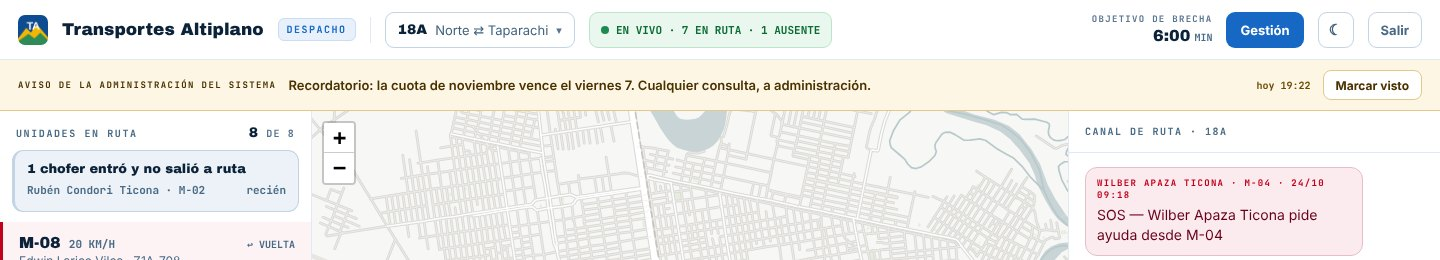
\includegraphics[width=\dimexpr\textwidth-2\fboxrule\relax]{img/d18-aviso-central}}
\end{center}

\section{El tema noche}

El botón de la luna pasa el panel a colores oscuros, para el turno de la noche;
el del sol lo devuelve. El panel recuerda la elección.

\pc{d06-noche}{El panel en el tema noche.}

\section{Gestión}

\boton{Gestión} abre el espacio de administración, con un menú a la izquierda
en tres grupos: \emph{Operación del día}, \emph{Ruta y medición} y \emph{La
cooperativa}. \boton{\texttimes\ Volver al mapa} regresa al panel.

\subsection{Personas}

Choferes, cobradores y las cuentas de Despacho y de gerencia. Se busca por
nombre, alias o unidad, y se filtra por rol.

\begin{itemize}
  \item \boton{+ Persona} abre el alta. Se elige \boton{CHOFER} o
    \boton{COBRADOR}, se escribe el nombre y apellido (con ese se liquidan las
    horas) y, si se quiere, el alias (así lo ven en el chat); la ruta, el
    usuario con el que va a entrar, la combi y la clave. \boton{$\circlearrowright$}
    genera una clave fácil de dictar. \boton{+ Alta} la crea.
  \item \boton{Clave} le pone una clave nueva. Su sesión abierta se cierra en
    el acto.
  \item \boton{Escribir} le abre un privado \textbf{sólo a esa persona} (ver
    \emph{Escribirle a una combi o a una persona}).
  \item \boton{Combis} marca las combis que puede manejar: entre ésas elige
    en la puerta, cada día. \rotulo{La de hoy} es en la que está ahora (no se
    le cambia a alguien en ruta). \boton{Cualquiera de su ruta} es para el
    suplente: puede salir en cualquier combi de su ruta sin habilitarlas una
    por una. En la lista, \rotulo{M-05 +1} quiere decir que hoy va en M-05 y
    tiene una más habilitada.
  \item \boton{Editar} corrige el nombre o el alias.
  \item \boton{Baja} la saca del sistema. Sus horas y vueltas quedan en los
    informes.
\end{itemize}

\pc{d08b-combis}{Las combis que puede manejar Rufino: la suya (la de hoy) y M-07.}

Así no hace falta una cuenta por combi ni prestar la clave: cada uno entra
con la suya, y las horas, las vueltas y el SOS quedan a su nombre en la combi
en la que fue.

\pc{d08-alta-persona}{El alta de una persona.}

\begin{nota}
Las combis (con su placa) las da de alta la \textbf{gerencia}: Despacho sube a
la persona a una combi que ya exista. La columna \rotulo{Última conexión} dice
\emph{nunca entró} a quien todavía no usó su cuenta.
\end{nota}

\pc{d07-personas}{La lista de personas.}

\subsection{Vehículos}

Las combis de la cooperativa, su placa, quién va arriba, quiénes la pueden
manejar, y su estado:
\enverde{n arriba} (hay gente con la app abierta), \enambar{en línea} (la
combi está en el mapa aunque nadie tenga la pantalla abierta) o
\rotulo{parada}.

El \textbf{supervisor} (la cuenta de Despacho sin ruta fija) puede
\textbf{pasar una combi a otra ruta} de la cooperativa con el selector de la
columna \rotulo{Ruta}. Pide confirmación: si la combi está andando, la vuelta a
medias se pierde, su gente pasa con ella y su turno sigue en la ruta nueva.

\pc{d09-vehiculos}{Los vehículos de la cooperativa.}

\subsection{Turnos}

Quién anduvo en qué combi, cuándo entró y salió, y cuánto tiempo estuvo en
ruta: \boton{Hoy}, \boton{Ayer} o \boton{Esta semana}. Un turno se abre cuando
la persona sube a su combi y se cierra cuando se va; un corte de señal corto no
lo parte en dos.

\pc{d10-turnos}{Los turnos del día.}

\subsection{Rutas}

Una tarjeta por ruta con:

\begin{itemize}
  \item \textbf{El objetivo de brecha}, \rotulo{a mano} o \rotulo{automático}.
    Con el automático, el sistema lo calcula como la vuelta promedio dividida
    por las combis en ruta; hasta juntar 3 vueltas sigue valiendo el número
    cargado a mano.
  \item \textbf{El recorrido cargado} (puntos y kilómetros) y
    \boton{Abrir trazador} para corregirlo.
  \item \textbf{Con qué trazado se mide}, si la ruta tiene más de uno (por
    ejemplo, el de los domingos o el de una obra). Cambiarlo pide confirmación:
    descarta las vueltas en curso, que se venían midiendo con el otro dibujo.
\end{itemize}

\pc{d11-rutas}{Las rutas de la cooperativa.}

\subsubsection*{El trazador}

El trazador permite corregir el recorrido sobre el mapa. Se elige el tramo
(\boton{Ida} o \boton{Vuelta}); un clic agrega un punto al final, arrastrar un
punto lo mueve y tocarlo lo borra. El primer punto es el paradero inicial
(\textbf{A}) y el último el final (\textbf{B}). También se puede importar un
GPX o GeoJSON, o cargar una \boton{Grabación de la calle}: el recorrido que
grabó un chofer con la app. Desde ahí mismo se le puede \textbf{pedir} a una
combi que grabe su próxima vuelta. Nada cambia hasta \boton{Guardar recorrido}.

\pc{d12-trazador}{El trazador de Despacho.}

\begin{importante}
Si el trazado que se está dibujando no es el que se usa para medir, el
trazador lo avisa arriba: lo que se guarde ahí no cambia las brechas de hoy.
\end{importante}

\subsection{Vueltas}

Las vueltas cerradas hoy en la ruta, cada una con cuándo salió y volvió, la
brecha promedio que mantuvo (con su barra de color, juzgada contra el
objetivo que regía cuando se cerró) y lo que duró. Arriba, el resumen: vueltas
cerradas, vuelta promedio (y la de ayer), brecha promedio, vueltas en pelotón,
idas y retornos.

\pc{d13-vueltas}{Las vueltas del día.}

\subsection{Dónde se traba}

En qué punto del recorrido y a qué hora se detienen las combis, y en qué tramo
se corta siempre la señal: es información de la \textbf{ruta}, no de un chofer.
Varias combis cortándose en la misma franja es un tramo sin antena; una sola,
un teléfono. Debajo, las \textbf{anomalías} que el sistema vio en las
posiciones (saltos imposibles, ausente en marcha, reloj corrido, GPS simulado o
impreciso), con lo que significa cada una. Se anotan para poder preguntar, no
para acusar.

\pc{d14-donde-se-traba}{Dónde se traba la ruta.}

\subsection{Informes}

Descargas en \textbf{CSV} (se abren en Excel) para un rango de fechas de hasta
90 días: vueltas y brechas, medias vueltas, turnos por persona (las horas que
se liquidan), salidas del recorrido, paradas y avisos de tráfico, cortes de
señal, anomalías, emergencias, el chat y la actividad del panel. Cada archivo
arranca diciendo el período, con qué se midió y en qué huso horario están las
horas.

\pc{d15-informes}{Los informes.}

\subsection{Empresa y Actividad}

\textbf{Empresa} muestra los datos de la cooperativa (los corrige la
gerencia). \textbf{Actividad} es el registro de todo lo que se hizo en el panel
de esta cooperativa: altas, cambios de clave, cambios de objetivo, SOS,
avisos del sistema; y del mando de las combis: \emph{tomó la combi que
manejaba} (un relevo) y \emph{salió a ruta solo en} (la app vio al chofer
manejando sin haber salido y nadie contestó el aviso). Sólo la de ustedes.

\pc{d17-actividad}{La actividad de la cooperativa.}

% ════════════════════════════════════════════════════════════════════════
\chapter{Gerencia}
\label{cap:gerencia}

La gerencia entra por el \textbf{mismo panel} que Despacho, con su propia
cuenta (la da de alta la central), y ve todo lo que ve Despacho. Además:

\begin{itemize}
  \item administra los \textbf{activos}: da de alta las combis con su placa, y
    corrige los datos y el logo de la empresa;
  \item tiene la pestaña \textbf{Números}, con el cumplimiento del período.
\end{itemize}

La cuenta de gerencia puede abarcar toda la cooperativa o una sola ruta.
Despacho no puede tocarla: buena parte de lo que mira la gerencia es el
trabajo de Despacho.

\section{Dar de alta una combi}

En \textbf{Vehículos}, la gerencia tiene el formulario de alta: el código de la
combi (el que se ve en el mapa, por ejemplo \emph{M-21}) y la placa o una
descripción. \boton{+ Vehículo} la crea en la ruta elegida.

\pc{g04-vehiculo-alta}{La gerencia da de alta una combi.}

\section{La empresa y su logo}

En \textbf{Empresa}, la gerencia corrige el nombre, el RUC y el contacto, y sube
el \textbf{logo} (PNG, JPG o WEBP; se achica solo). El logo es lo que ven los
choferes y el panel: es la señal de que el sistema es de su cooperativa. Sin
logo se muestran las iniciales.

\pc{g03-empresa}{Los datos y el logo de la cooperativa.}

\section{Números}

Los números del período —\boton{7 días}, \boton{14 días} o \boton{30 días}—,
de toda la cooperativa o de una ruta. Un «día» es un día de calendario: «7
días» son los últimos siete contando hoy.

\begin{itemize}
  \item \textbf{Arriba}, las cifras del período: vueltas, idas, retornos,
    \textbf{cumplimiento} (el porcentaje de vueltas cuya brecha promedio estuvo
    en objetivo), brecha promedio, horas trabajadas, unidades activas, salidas
    del recorrido, cortes de señal, horas sin señal, horas ausente, paradas y
    SOS.
  \item \textbf{Por unidad}: cada combi con sus vueltas, cumplimiento, brecha
    promedio, duración (y la mejor), velocidad promedio, horas y salidas.
  \item \textbf{Por persona}: las horas que se liquidan, con los turnos, las
    vueltas y el cumplimiento de cada uno. Las vueltas se le atribuyen al
    chofer que iba manejando.
  \item Más abajo, la tendencia por día y la señal y presencia de cada combi.
\end{itemize}

Cada vuelta se juzga contra el objetivo que regía cuando se cerró, no contra
el de hoy. Los botones \boton{CSV vueltas}, \boton{CSV turnos} y los demás
bajan lo mismo para una planilla.

\pc{g01-numeros}{Números: las cifras del período y la tabla por unidad.}
\pc{g02-numeros-tablas}{Números: la tabla por persona, con las horas que se liquidan.}

% ════════════════════════════════════════════════════════════════════════
\chapter{La central}
\label{cap:central}

La central es el nivel de arriba de todas las cooperativas: quien vende,
instala y mantiene el sistema. Su panel es una herramienta interna: sobria, sin
marca y sin «recordarme».

\section{Entrar}

El panel de la central sólo existe si el servidor tiene configurada su clave;
si no, su dirección no responde. Pide la \textbf{clave} y, si está configurado,
el \textbf{código del segundo factor} (de una app de autenticación). La sesión
muere al cerrar la pestaña.

\pc[0.6]{k01-creador-entrar}{La entrada al panel de la central.}

\section{Cooperativas}

La lista de cooperativas, cada una con sus rutas, sus combis, su gente, las
\emph{unidades-día} del mes (cuántas combis trabajaron cuántos días: es lo que
se cobra), su última señal y sus cuentas.

\pc{k02b-cooperativas}{Las cooperativas del sistema.}

\subsection{Una cooperativa nueva}

\boton{+ Nueva cooperativa} pide el \textbf{código} (no se puede cambiar
después: de él cuelga todo), el nombre, el RUC y el contacto, la
\textbf{primera ruta} con su nombre, y la \textbf{cuenta de Despacho} con su
clave. La ruta y la cuenta son opcionales, pero conviene cargarlas acá: sin
ruta nadie se puede conectar y sin Despacho no hay quién administre. La clave
se ve una sola vez: hay que anotarla para dictarla.

\pc{k03-nueva-cooperativa}{El alta de una cooperativa.}

\subsection{Administrar}

\boton{Administrar} abre la tarjeta de una cooperativa:

\begin{itemize}
  \item \textbf{Datos}: nombre, RUC y contacto.
  \item \textbf{Logo}: el mismo que puede subir su gerencia.
  \item \textbf{Aviso a la cooperativa}: un mensaje que aparece como franja
    ámbar en su panel de Despacho hasta que alguien lo marque visto (por
    ejemplo, un pago pendiente). Puede ir a una sola ruta. No toca el chat de
    los choferes.
  \item \textbf{Cuenta de Despacho}: crearla o restablecerle la clave (sus
    sesiones abiertas se cierran). Queda en la actividad de esa cooperativa.
  \item \textbf{Ruta nueva}: el código y el nombre; el recorrido se dibuja
    después, en \boton{RUTAS}.
  \item \textbf{Cuenta de gerencia}: crearla o restablecerla, con alcance a
    toda la cooperativa o a una ruta.
\end{itemize}

\pc{k09-aviso}{La tarjeta de una cooperativa, con un aviso pendiente.}

\subsection{Suspender}

\boton{Suspender} saca de circulación a una cooperativa entera \textbf{en el
acto}: se cierran todas sus sesiones y nadie de ella puede entrar. La
confirmación dice el nombre de la cooperativa que se va a suspender. Se puede
reactivar.

\section{Rutas: los trazados}

En \boton{RUTAS} se eligen la cooperativa, la ruta y el \textbf{trazado}. Acá
se dibujan los recorridos al dar de alta una cooperativa (Despacho a lo sumo
corrige).

\begin{itemize}
  \item Las herramientas: \boton{DIBUJAR}, \boton{MANO} (o la barra
    espaciadora), \boton{SELECCIONAR} (dos clics borran el tramo entre ellos),
    \boton{IDA} y \boton{VUELTA}, \boton{Deshacer} (o Ctrl+Z) e
    \boton{Importar GPX}. Un clic sobre la línea inserta un punto en el medio.
  \item \boton{+ Nuevo trazado} crea otro dibujo para la misma ruta (el de los
    domingos, el de una obra), con vigencia por fechas, por días de la semana
    o las dos cosas: rige solo en esos días y vuelve solo al de siempre.
  \item \boton{Renombrar ruta} corrige el nombre que ven todos.
\end{itemize}

\pc{k05-trazador}{El trazador de la central, con la ida de la 18A.}

\section{Respaldos}

El sistema respalda la base cada 6 horas y conserva los últimos 28.
\boton{Respaldar ahora} hace uno en el momento y \boton{Descargar} lo baja:
\textbf{el archivo guardado en otra máquina es el respaldo que sobrevive a
perder el servidor}. Conviene bajar uno cada tanto.

\pc{k06-respaldos}{Los respaldos de la base.}

\section{Sistema}

La salud del servidor: hace cuánto está encendido, el último respaldo, las
unidades en el mapa, las conexiones, cooperativas, rutas, combis y personas, el
tamaño de la base y la memoria. Arriba, los avisos de riesgo:

\begin{itemize}
  \item \enrojo{RIESGO DE PÉRDIDA}: la base está en el mismo disco que la
    aplicación. En un servidor que se redespliega, ese disco se borra.
  \item \enambar{UN SOLO FACTOR}: el panel entra sólo con clave. Es el nivel
    que puede crear y suspender cooperativas.
\end{itemize}

\pc{k07-sistema}{La salud del sistema.}

\section{Actividad}

Lo que pasó en todas las cooperativas juntas: es el único lugar del sistema
donde se ven así. Las acciones de la central figuran como \textbf{CREADOR}.

\pc{k08-actividad}{La actividad de todas las cooperativas.}

% ════════════════════════════════════════════════════════════════════════
\chapter{Problemas frecuentes}
\label{cap:problemas}

\begin{description}[leftmargin=0pt,labelsep=0.6em,itemsep=6pt]
  \item[«No tengo brecha».] Si la pantalla dice \enambar{YENDO A LA RUTA}, el
    GPS todavía no vio la combi sobre el recorrido: arranca solo al pisarlo. Si
    dice \emph{sin nadie}, no hay otra combi en la cadena de ese tramo.
  \item[«Mi combi no aparece en el mapa de Despacho».] Revisar que el
    celular tenga la ubicación activada y el permiso dado (la web lo dice en
    rojo: \enrojo{SIN GPS}). En la app Android, revisar la optimización de
    batería (sección \ref{sec:android}).
  \item[«Dice que otro chofer tomó la unidad».] Dos personas entraron en la
    misma combi: manda el GPS del último que entró. El otro sigue viendo
    todo, pero su posición no se usa.
  \item[«Aparece SIN SEÑAL pero tengo internet».] Si Despacho ve \emph{el
    teléfono sigue mandando}, el celular manda posiciones viejas: reiniciar la
    app suele bastar.
  \item[«Me marcó ENTRÓ 40\,\%».] La combi se metió a la ruta ya empezada. Esa
    primera vuelta queda como parcial y no cuenta en los promedios; las
    siguientes, sí.
  \item[«Me olvidé la clave».] La de un chofer o un cobrador la cambia
    Despacho (Gestión \flecha Personas \flecha \boton{Clave}); la de un
    cobrador, también el chofer desde la app Android. La de Despacho y la de
    gerencia, la central.
  \item[«Salí de ruta sin querer».] Volver a entrar y tocar
    \boton{SALIR A RUTA}. La vuelta que se llevaba se perdió.
  \item[«Mandé un SOS por error».] Avisar enseguida por el chat a Despacho. En
    Despacho, \boton{ATENDIDO} saca la alerta.
\end{description}

% ════════════════════════════════════════════════════════════════════════
\chapter{Glosario}

\begin{description}[leftmargin=0pt,labelsep=0.6em,itemsep=3pt]
  \item[Brecha.] Minutos de recorrido entre una combi y la de adelante o la de
    atrás, en el mismo tramo.
  \item[Cadena.] Las combis que están en ruta y confirmadas sobre el
    recorrido: las que se miden entre sí.
  \item[Cumplimiento.] Porcentaje de vueltas cuya brecha promedio estuvo en
    objetivo.
  \item[Entrada tardía.] Meterse a la ruta más allá del 15\,\% del circuito.
    La primera vuelta queda parcial.
  \item[Objetivo de brecha.] La separación ideal entre combis de una ruta, a
    mano o automática.
  \item[Pelotón.] Combis pegadas una a la otra (brecha crítica por poca
    separación).
  \item[Presencia.] Lo que declara el chofer: en ruta, ausente o fuera.
  \item[Supervisor.] La cuenta de Despacho sin ruta fija: ve todas las rutas de
    la cooperativa y puede pasar combis de una a otra.
  \item[Trazado.] Un dibujo del recorrido de una ruta (ida y retorno). Una ruta
    puede tener varios y medirse con uno a la vez.
  \item[Tramo.] La ida o el retorno.
  \item[Unidades-día.] Cuántas combis trabajaron cuántos días en el mes.
  \item[Vuelta.] El circuito completo, ida y retorno.
\end{description}

\end{document}
